\section{Results}
\label{sec:results}
The results first describe the UNI2-h experiment on its own, with the endpoints of the Virchow2 study, and then compare the two encoders through the pre-specified paired contrast and the conclusions of the Virchow2 study.

\subsection{Damage under UNI2-h}
The balanced CE model reaches 72.45 percent BA $[71.15, 73.60]$, 0.94 points above its Virchow2 counterpart. At $\rho=100$ it reaches 69.95 percent $[68.68, 71.06]$, the same point estimate as under Virchow2, so it loses $D_{100}=2.49$ points $[2.01, 2.94]$ against Virchow2's 1.56. UNI2-h's advantage on balanced data thus disappears under imbalance. The frozen UNI2-h readout lost a similar 2.29 points, from a balanced BA of 73.98 percent to 71.69 percent at $\rho=100$. The LoRA model is 1.53 points less accurate than the frozen readout on balanced data and 1.74 points less accurate at $\rho=100$. Under Virchow2, the LoRA model was 0.55 points less accurate than the frozen readout on balanced data but 0.81 points more accurate at $\rho=100$, which halved its damage. Adapting UNI2-h with this recipe does not reproduce that reduction. The frozen values come from different draws and are descriptive.

\subsection{Recovery per method}
Figure~\ref{fig:recovery} and Table~\ref{tab:recovery} give each method's paired recovery under UNI2-h. Four of eight variants recover a material part of the damage: CUDA (1.79 points $[1.43, 2.17]$), train-time logit adjustment (1.61 $[1.26, 1.98]$), post-hoc logit adjustment (1.51 $[1.28, 1.74]$), and balanced sampling (1.18 $[0.88, 1.47]$). End-to-end GCL (0.88), DisAlign (0.73), classifier-only GCL (0.71), and cRT (0.68) show positive recoveries below the one-point threshold. CUDA's share of the damage, 0.72 $[0.58, 0.89]$, is the largest, followed by the two forms of logit adjustment (0.65 and 0.60). No share interval reaches 1. CUDA and both forms of logit adjustment meet the pre-specified full-recovery criterion: their marginal accuracy intervals, which span about 2.5 points, contain the balanced CE point estimate of 72.45 percent. This criterion is less informative than the paired shares, whose upper bounds remain below 1. The point estimates leave between 0.28 and 0.40 of the damage unrecovered.

\begin{figure}[t]
  \centering
  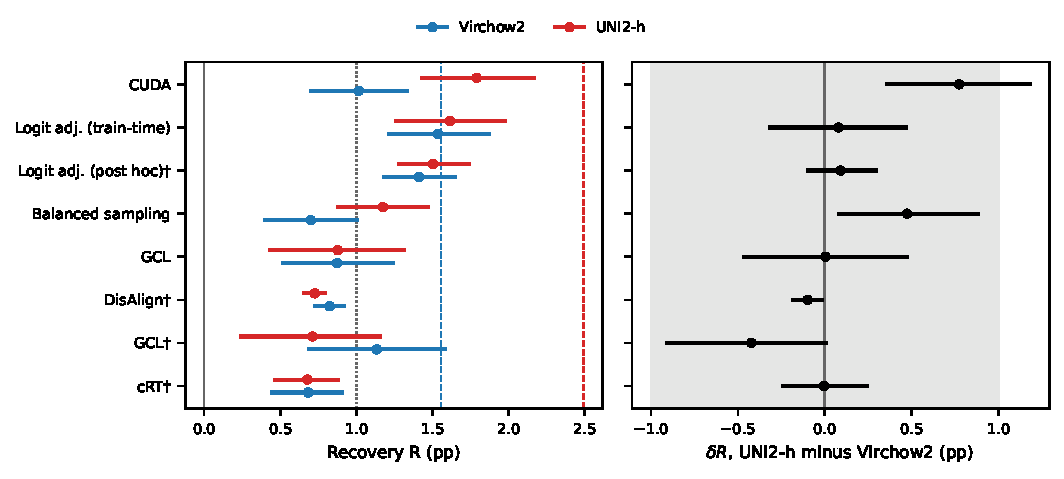
\includegraphics[width=\textwidth]{fig_recovery.pdf}
  \caption{Under UNI2-h, CUDA recovers more than under Virchow2, and the other recoveries change by less than half a point, while the damage they are measured against grows. Left: paired recovery $R_m$ at $\rho=100$ with 95\% intervals for Virchow2 (blue) and UNI2-h (red); dashed lines mark each encoder's CE damage $D_{100}$, the solid line zero, and the dotted line the one-point threshold. Right: paired contrast $\delta R_m$ (UNI2-h minus Virchow2) with 95\% intervals; the grey band marks $\pm1$ point. $^{\dagger}$Classifier only.}
  \label{fig:recovery}
\end{figure}

\begin{table}[t]
\centering
\small
\begin{tabular}{@{}lccc@{}}
\toprule
Method & $R_m$ & share & $\mathrm{BA}(m^{*},100)$ \\
\midrule
CUDA & \textbf{1.79} $[1.43, 2.17]$ & 0.72 $[0.58, 0.89]$ & 71.74 $[70.47, 72.81]$ \\
Logit adj.\ (train-time) & \textbf{1.61} $[1.26, 1.98]$ & 0.65 $[0.54, 0.76]$ & 71.57 $[70.24, 72.74]$ \\
Logit adj.\ (post hoc)$^{\dagger}$ & \textbf{1.51} $[1.28, 1.74]$ & 0.60 $[0.52, 0.72]$ & 71.46 $[70.16, 72.58]$ \\
Balanced sampling & \textbf{1.18} $[0.88, 1.47]$ & 0.47 $[0.37, 0.59]$ & 71.13 $[69.87, 72.30]$ \\
GCL & 0.88 $[0.43, 1.31]$ & 0.35 $[0.20, 0.49]$ & 70.83 $[69.54, 72.04]$ \\
DisAlign$^{\dagger}$ & 0.73 $[0.66, 0.80]$ & 0.29 $[0.25, 0.35]$ & 70.68 $[69.38, 71.78]$ \\
GCL$^{\dagger}$ & 0.71 $[0.24, 1.16]$ & 0.29 $[0.11, 0.42]$ & 70.67 $[69.40, 71.81]$ \\
cRT$^{\dagger}$ & 0.68 $[0.47, 0.88]$ & 0.27 $[0.20, 0.35]$ & 70.63 $[69.33, 71.71]$ \\
\midrule
CE, balanced & -- & -- & 72.45 $[71.15, 73.60]$ \\
CE, $\rho=100$ & -- & -- & 69.95 $[68.68, 71.06]$ \\
\bottomrule
\end{tabular}
\caption{Under UNI2-h, four variants recover at least one point at $\rho=100$, and no share interval reaches the full damage of $D_{100}=2.49$ points. Recovery $R_m$ in BA points, its share of the CE damage, and the method's BA in percent, with paired 95\% intervals for $R_m$ and share and unpaired intervals for BA; bold marks material recovery ($R_m\geq1$, interval above zero). $^{\dagger}$Classifier only, frozen encoder; unmarked rows train end to end.}
\label{tab:recovery}
\end{table}

\subsection{Imbalance-specific recovery}
Table~\ref{tab:specific} separates each method's effect on balanced data from its imbalance correction. CUDA improves the balanced model by $G=0.70$ points $[0.34, 1.07]$, close to its 0.81 points under Virchow2. cRT loses 0.56 points $[-0.69, -0.45]$, and DisAlign is indistinguishable from CE. Both GCL forms lose more balanced accuracy than under Virchow2: 1.45 points $[-1.80, -1.11]$ end to end and 1.67 points $[-2.03, -1.32]$ classifier only.

After subtracting the balanced gains, the two GCL forms correct the most imbalance: 2.38 points $[1.82, 2.95]$ classifier only and 2.33 points $[1.77, 2.86]$ end to end, shares of 0.96 and 0.93 whose intervals include 1. Both models lose less than 0.2 points of their own balanced accuracy at $\rho=100$. Their recovery against CE stays below one point only because they start from a lower balanced accuracy. cRT corrects 1.24 points $[1.02, 1.47]$. CUDA's imbalance-specific recovery, 1.09 points $[0.64, 1.54]$ or a share of 0.44, is material under UNI2-h, whereas under Virchow2 its interval included zero (0.20 points $[-0.17, 0.57]$). DisAlign's 0.72 points stay below the threshold.

\begin{table}[t]
\centering
\small
\begin{tabular}{@{}lccc@{}}
\toprule
Method & $G_m$ & $R_m-G_m$ & share of $R_m-G_m$ \\
\midrule
GCL$^{\dagger}$ & $-1.67$ $[-2.03, -1.32]$ & \textbf{2.38} $[1.82, 2.95]$ & 0.96 $[0.81, 1.10]$ \\
GCL & $-1.45$ $[-1.80, -1.11]$ & \textbf{2.33} $[1.77, 2.86]$ & 0.93 $[0.79, 1.09]$ \\
cRT$^{\dagger}$ & $-0.56$ $[-0.69, -0.45]$ & \textbf{1.24} $[1.02, 1.47]$ & 0.50 $[0.42, 0.60]$ \\
CUDA & 0.70 $[0.34, 1.07]$ & \textbf{1.09} $[0.64, 1.54]$ & 0.44 $[0.29, 0.57]$ \\
DisAlign$^{\dagger}$ & 0.01 $[0.00, 0.01]$ & 0.72 $[0.65, 0.79]$ & 0.29 $[0.25, 0.35]$ \\
\bottomrule
\end{tabular}
\caption{Under UNI2-h, both GCL forms correct almost the full imbalance damage net of their balanced loss, and CUDA's imbalance-specific recovery is material. Balanced gain $G_m$ and imbalance-specific recovery $R_m-G_m$ (Eq.~\ref{eq:endpoints}) at $\rho=100$ in BA points, with the latter's share of the CE damage; paired 95\% intervals, bold marks material recovery. $^{\dagger}$Classifier only. Balanced sampling and logit adjustment have $G_m=0$ by construction, so their $R_m$ in Table~\ref{tab:recovery} is already imbalance-specific.}
\label{tab:specific}
\end{table}

\subsection{Encoder contrast}
One of the 20 pre-specified quantities meets the rule for encoder dependence: the balanced gain of classifier-only GCL, which is 1.07 points lower under UNI2-h $[-1.58, -0.59]$ (Table~\ref{tab:contrast}). End-to-end GCL's balanced gain falls by a similar 0.90 points $[-1.39, -0.43]$, just below the one-point threshold.

Nine further contrasts have intervals that exclude zero but magnitudes below one point. Two of them describe CE itself: UNI2-h's balanced model is 0.94 points more accurate $[0.45, 1.38]$, and its damage is 0.94 points larger $[0.47, 1.40]$. Because both CE models reach the same accuracy at $\rho=100$, each recovery contrast $\delta R_m$ equals the difference in the method's own accuracy at $\rho=100$. CUDA recovers 0.77 points more $[0.36, 1.18]$ and balanced sampling 0.47 points more $[0.08, 0.88]$. Logit adjustment, end-to-end GCL, and cRT recover within 0.1 points of their Virchow2 values, with intervals that include zero. Classifier-only GCL recovers 0.42 points less, with an interval that just includes zero, $[-0.91, 0.01]$. The imbalance-specific recoveries of CUDA (0.88 points $[0.28, 1.45]$) and end-to-end GCL (0.90 points $[0.25, 1.54]$) are larger under UNI2-h; that of classifier-only GCL is larger by 0.65 points with an interval that just includes zero. DisAlign's recovery and imbalance-specific recovery are about 0.1 points smaller, with intervals that exclude zero.

\begin{table}[t]
\centering
\small
\begin{tabular}{@{}llccc@{}}
\toprule
Quantity & Method & Virchow2 & UNI2-h & $\delta$ (UNI2-h $-$ Virchow2) \\
\midrule
$\mathrm{BA}(\mathrm{CE},1)$ & -- & 71.51 & 72.45 & $0.94$ $[0.45, 1.38]$ \\
$D_{100}$ & -- & 1.56 & 2.49 & $0.94$ $[0.47, 1.40]$ \\
\midrule
$R_m$ & CUDA & 1.02 & 1.79 & $0.77$ $[0.36, 1.18]$ \\
 & Logit adj.\ (train-time) & 1.54 & 1.61 & $0.08$ $[-0.31, 0.47]$ \\
 & Logit adj.\ (post hoc)$^{\dagger}$ & 1.41 & 1.51 & $0.09$ $[-0.10, 0.29]$ \\
 & Balanced sampling & 0.70 & 1.18 & $0.47$ $[0.08, 0.88]$ \\
 & GCL & 0.87 & 0.88 & $0.01$ $[-0.47, 0.47]$ \\
 & DisAlign$^{\dagger}$ & 0.83 & 0.73 & $-0.10$ $[-0.18, -0.02]$ \\
 & GCL$^{\dagger}$ & 1.13 & 0.71 & $-0.42$ $[-0.91, 0.01]$ \\
 & cRT$^{\dagger}$ & 0.68 & 0.68 & $-0.00$ $[-0.24, 0.24]$ \\
\midrule
$G_m$ & CUDA & 0.81 & 0.70 & $-0.11$ $[-0.54, 0.34]$ \\
 & GCL & $-0.55$ & $-1.45$ & $-0.90$ $[-1.39, -0.43]$ \\
 & GCL$^{\dagger}$ & $-0.60$ & $-1.67$ & $\mathbf{-1.07}$ $[-1.58, -0.59]$ \\
 & cRT$^{\dagger}$ & $-0.41$ & $-0.56$ & $-0.15$ $[-0.33, 0.01]$ \\
 & DisAlign$^{\dagger}$ & $-0.00$ & $0.01$ & $0.01$ $[-0.00, 0.02]$ \\
\midrule
$R_m-G_m$ & CUDA & 0.20 & 1.09 & $0.88$ $[0.28, 1.45]$ \\
 & GCL & 1.42 & 2.33 & $0.90$ $[0.25, 1.54]$ \\
 & GCL$^{\dagger}$ & 1.73 & 2.38 & $0.65$ $[-0.00, 1.30]$ \\
 & cRT$^{\dagger}$ & 1.10 & 1.24 & $0.14$ $[-0.11, 0.43]$ \\
 & DisAlign$^{\dagger}$ & 0.83 & 0.72 & $-0.11$ $[-0.19, -0.03]$ \\
\bottomrule
\end{tabular}
\caption{Only classifier-only GCL's balanced gain meets the encoder-dependence rule (bold); nine further contrasts exclude zero at less than one point. Point estimates per encoder at $\rho=100$ in BA points and the paired contrast $\delta$ (Eq.~\ref{eq:delta}) with its 95\% interval. $^{\dagger}$Classifier only.}
\label{tab:contrast}
\end{table}

Method rankings change despite the small recovery contrasts. Six of eight material-recovery verdicts agree between encoders. The two that differ lie near the threshold: balanced sampling is material only under UNI2-h (0.70 against 1.18 points) and classifier-only GCL only under Virchow2 (1.13 against 0.71 points). The Spearman correlation of $R_m$ across the eight variants is 0.57. All eight recoveries lie between 0.68 and 1.79 points under both encoders, so a shift of a few tenths of a point reorders them.

\subsection{Conclusions of the Virchow2 study}
Table~\ref{tab:claims} checks six conclusions of the Virchow2 study at $\rho=100$. Three carry over to UNI2-h. Logit adjustment and classifier-only GCL remain the methods that restore most of the tail recall (Section~\ref{sec:rank}). Post-hoc logit adjustment again recovers nearly as much as its train-time form, 1.51 against 1.61 points. Classifier-only GCL again gives the largest imbalance-specific recovery, only 0.05 points ahead of end-to-end GCL. Three do not carry over. Logit adjustment no longer has paired recovery shares compatible with 1: its shares of 0.65 and 0.60 have upper bounds of 0.76 and 0.72, and CUDA now gives the largest recovery. Both forms still meet the marginal-interval full-recovery criterion; the conclusion here concerns the paired shares. CUDA's imbalance-specific recovery is material, so its gain is no longer purely general. Finally, the LoRA model is no longer less sensitive to imbalance than the frozen readout. Differences between methods are not tested, and the frozen comparison is descriptive.

\begin{table}[t]
\centering
\small
\renewcommand{\arraystretch}{1.15}
\begin{tabularx}{\textwidth}{@{}>{\raggedright\arraybackslash}p{0.27\textwidth}YY>{\raggedright\arraybackslash}p{0.10\textwidth}@{}}
\toprule
Conclusion at $\rho=100$ & Virchow2 & UNI2-h & Verdict \\
\midrule
(i) Logit adjustment gives the largest $R_m$ and its paired share interval contains 1 & 1.54 (train-time), share 0.99 $[0.80, 1.24]$ & 1.61, share 0.65 $[0.54, 0.76]$; CUDA 1.79 & Fails \\
(ii) Logit adjustment and GCL$^{\dagger}$ restore most of the tail recall & Tail 61.2 to 69.4, 69.9, and 72.2; others $\leq$66.6 & Tail 60.0 to 68.9, 69.3, and 69.5; others $\leq$67.5 & Holds \\
(iii) Post-hoc logit adjustment matches its train-time form & 1.41 vs.\ 1.54 & 1.51 vs.\ 1.61 & Holds \\
(iv) CUDA's gain is general ($R_m-G_m$ includes 0) & 0.20 $[-0.17, 0.57]$ & 1.09 $[0.64, 1.54]$ & Fails \\
(v) GCL$^{\dagger}$ gives the largest $R_m-G_m$ & 1.73; next 1.42 (GCL) & 2.38; next 2.33 (GCL) & Holds \\
(vi) LoRA damage smaller than the frozen readout's & 1.56 vs.\ 2.91 & 2.49 vs.\ 2.29 & Fails \\
\bottomrule
\end{tabularx}
\caption{Three of six conclusions of the Virchow2 study carry over to UNI2-h; logit adjustment's paired share intervals exclude 1, CUDA's gain is partly imbalance-specific, and LoRA no longer reduces the damage. Values in BA points or recall points; tail recall is the patient-macro recall of the rarest third of classes for CE, the two logit-adjustment forms, and classifier-only GCL. The frozen readouts in (vi) come from the same draws for Virchow2 and from different draws for UNI2-h. $^{\dagger}$Classifier only.}
\label{tab:claims}
\end{table}

\subsection{Recovery by class rank}
\label{sec:rank}
Under UNI2-h, the CE model at $\rho=100$ keeps 60.0 percent recall in the tail third of classes by assigned rank, against 72.9 percent when balanced, and gains 6.6 points in the head (Figure~\ref{fig:rank}). The tail thus loses 13.0 points, against 10.4 under Virchow2. Logit adjustment raises the tail to 68.9 (train-time) and 69.3 percent (post hoc), at a cost of four to five points of head recall. Classifier-only GCL raises it to 69.5 percent with a head recall of 71.6 percent, close to the balanced model's 72.1; under Virchow2 its tail recall exceeded the balanced model's, whereas here it stays 3.4 points below. End-to-end GCL follows at 67.5 percent. CUDA, balanced sampling, cRT, and DisAlign leave the tail between 62.9 and 64.9 percent and the head between 75.7 and 77.9 percent; CUDA instead gains in the body, 72.6 against CE's 71.2 percent. Each method thus recovers recall in the same rank group as under Virchow2. Rank-group recalls are point estimates.

\begin{figure}[t]
  \centering
  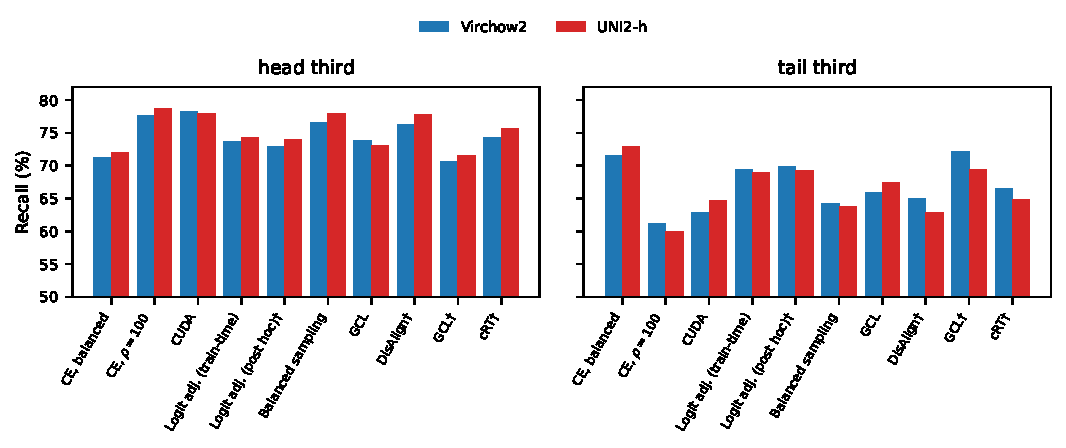
\includegraphics[width=\textwidth]{fig_rank_recall.pdf}
  \caption{Under both encoders, logit adjustment and classifier-only GCL restore most of the tail recall at $\rho=100$, at the cost of head recall; CUDA and balanced sampling keep the head-heavy profile of CE. Patient-macro recall of the head and tail thirds of classes by assigned rank, averaged over shards, for Virchow2 (blue) and UNI2-h (red). $^{\dagger}$Classifier only.}
  \label{fig:rank}
\end{figure}

\subsection{Selected strengths and probability quality}
Validation selects stronger prior corrections under UNI2-h. Train-time logit adjustment selects the full correction $\tau=1$ in 21 of 30 shards and its post-hoc form in 24, whereas under Virchow2 half the correction, $\tau=0.5$, was selected in 17 and 20 shards. Balanced sampling selects full balancing ($s=1$) in 25 of 30 shards (Virchow2: 19). CUDA selects its lowest augmentation probability, $p_{\mathrm{aug}}=0.25$, in 18 of 30 shards at $\rho=100$ and in 21 on the balanced allocation, and never selects 1. End-to-end GCL selects $\sigma=0.05$ in 20 of 30 shards; its classifier-only form selects the lowest value, $\sigma=0.01$, in 15. DisAlign selects the largest value in its grid, $\gamma=2$, in 22 of 30 shards, whereas under Virchow2 $\gamma=1.5$ was selected in 19 shards.

Imbalance worsens the raw probabilities slightly under UNI2-h. Both CE models are overconfident: their validation temperatures average 1.80 (balanced) and 1.69 ($\rho=100$), similar to Virchow2's 1.86 and 1.70 and unlike the underconfident frozen UNI2-h readout. From the balanced allocation to $\rho=100$, raw NLL rises from 1.37 to 1.43 nats and raw ECE from 17.9 to 18.2 points; after temperature scaling, NLL rises from 1.03 to 1.13 nats and ECE from 4.1 to 5.1 points. CUDA has the lowest raw NLL, 1.07 nats $[1.01, 1.14]$, and raw ECE, 11.4 points $[10.4, 12.5]$; end-to-end GCL (1.68 nats) and cRT (1.48) have the highest raw NLL. After temperature scaling, NLL ranges from 0.98 (CUDA) to 1.12 nats (end-to-end GCL) against CE's 1.13, and ECE from 2.6 (post-hoc logit adjustment) to 4.7 points (balanced sampling) against CE's 5.1. The scaled intervals are unpaired and overlap. As under Virchow2, CUDA curbs raw overconfidence, and temperature scaling brings the other methods close to it.

\section{Discussion}
\label{sec:discussion}
\textbf{Does mitigation under LoRA depend on the encoder?} Most recovery contrasts are small. Among the 20 pre-specified quantities, only classifier-only GCL's balanced gain meets the encoder-dependence rule, and at $\rho=100$ seven of eight methods reach within half a point of their Virchow2 accuracy. The reference accuracy changes. UNI2-h's balanced CE model is about one point more accurate, but its $\rho=100$ model is not, so the damage grows by about one point. Measured against that larger damage, recoveries that stay the same in points become smaller shares, and logit adjustment's paired share intervals exclude full recovery. The material-recovery verdicts of balanced sampling and classifier-only GCL change because their estimates lie near one point, not because their contrasts meet the encoder-dependence rule. The conclusions of the Virchow2 study \citep{queisler2026mitigationTcga} that concern where methods act transfer: logit adjustment and classifier-only GCL restore the tail, post-hoc correction matches train-time correction, and GCL corrects the most imbalance net of its balanced loss. The conclusions that concern how much of the damage is recovered do not.

\textbf{Why does CUDA's imbalance-specific recovery become material?} CUDA's own damage is the accuracy it loses from the balanced allocation to $\rho=100$. It is similar under both encoders (1.41 and 1.35 points), as is CUDA's balanced gain. CE's damage grows by 0.94 points, so the difference between the two damages, CUDA's imbalance-specific recovery, grows by about the same amount. GCL behaves the same way: under both encoders it loses less than 0.2 points to imbalance, and its imbalance-specific recovery grows with CE's damage. Logit adjustment, cRT, and DisAlign instead lose 0.8 to 1.0 points more to imbalance under UNI2-h, so their recoveries stay flat. These own-damage values are point estimates without intervals. On BRACS, CUDA's imbalance-specific recovery also became material under UNI2-h, with an unresolved contrast of 0.51 points \citep{queisler2026mitigationUni2h}; on TCGA-UT the contrast of 0.88 points excludes zero. Across both datasets, CUDA's gain is therefore not purely general under UNI2-h, but whether it corrects imbalance by itself or merely resists the greater damage that CE suffers with this encoder cannot be separated with these endpoints.

\textbf{Why does GCL lose more on balanced data?} With a uniform class prior, all of GCL's clouds have the same size and GCL reduces to CE with a cosine head, so its balanced loss reflects the cosine head and its fixed scale $s=30$ rather than any imbalance correction. That loss is 0.9 to 1.1 points larger under UNI2-h. The scale and noise level were taken from the reference implementation and the Virchow2 grid; UNI2-h's adapted features may have different norms and angular spread, so the same scale may fit this encoder less well. The design does not test this explanation.

\textbf{How large a difference could have been missed?} Much less than on BRACS. The paired intervals of the recovery contrasts span 0.16 to 0.94 points and those of the imbalance-specific recoveries up to 1.31 points, against up to four points on BRACS \citep{queisler2026mitigationUni2h}. Of the 20 quantities, 12 have intervals that lie entirely within $\pm1$ point, including all recoveries except CUDA's; these intervals exclude encoder effects of one point in either direction. The other eight intervals reach beyond one point: the balanced accuracy, the damage, CUDA's recovery, both GCL balanced gains, and the imbalance-specific recoveries of CUDA and both GCL forms. This equivalence reading was not pre-specified and is descriptive.

\textbf{Does UNI2-h change the frozen-versus-LoRA picture?} Yes. Under Virchow2, adaptation made the imbalanced model 0.81 points more accurate than the frozen readout and halved the damage. Under UNI2-h, the LoRA model is less accurate than the frozen readout on both allocations, and its damage, 2.49 points, is as large as the frozen readout's 2.29. The best mitigated UNI2-h model at $\rho=100$, CUDA at 71.74 percent, stays 2.24 points below the frozen UNI2-h readout on balanced data and only matches the frozen readout at $\rho=100$ (71.69 percent). For TCGA-UT, adapting UNI2-h with the recipe tuned for Virchow2 and then mitigating does not improve on a frozen UNI2-h readout. The frozen values come from different draws.

\textbf{Limitations.} The study adds a second encoder but keeps one dataset, one adaptation scheme, and one imbalance ratio; the contrast at $\rho=50$ and at native class shares is not measured. All settings were tuned under Virchow2 and transferred unchanged: the 2,400 training steps, the LoRA rank and target modules, GCL's scale, and the strength grids. This keeps the comparison paired, but it measures UNI2-h under a recipe tuned for the other encoder, and UNI2-h's 1.53-point gap to its own frozen readout may partly reflect that. Three methods frequently select grid endpoints: DisAlign's largest $\gamma$ (22 of 30 shards), CUDA's lowest $p_{\mathrm{aug}}$ (18), and classifier-only GCL's lowest $\sigma$ (15). The grids were not extended, so these methods' recoveries, and DisAlign's small negative contrasts, may partly reflect truncation. The encoders also differ in their pooled embedding (1,536 against 2,560 dimensions), so the contrast describes two complete encoder-plus-pooling pipelines. The UNI2-h fits accumulate gradients over four micro-batches of 64 patches into the same 256-patch update and use compiled kernels; in a short run on one shard, compiled and uncompiled training differed by 0.35 points of validation BA, less than the 0.88 points between two uncompiled repeats. Imbalance-specific recovery assumes that a method's balanced effect carries over additively to the imbalanced allocation. The comparisons with the frozen readouts and with BRACS are descriptive.
